\documentclass[12pt]{article}
\usepackage[utf8]{inputenc}
\usepackage[spanish]{babel}
\usepackage{amsmath} 
\usepackage{amsfonts}
\usepackage{graphicx}


\newenvironment{micaja}
{
    \begin{center}
    \begin{tabular}{|p{0.9\textwidth}|}
    \hline\\
    }   
    {   
    \\\\\hline
    \end{tabular} 
    \end{center}
    }



\title{Control 1}
\author{Blanca Cano Camarero}
\begin{document}
\begin{titlepage}
\maketitle
\tableofcontents
\end{titlepage}

\section{Ejercicio 1}
En el grupo simétrico $S_8$ se consideran los elementos
\begin{equation*}
    \pi = (145)(283)(67) \text{ y } 
    \beta = \begin{pmatrix}
      1 & 2 & 3 & 4 & 5 & 6 & 7 & 8 \\ 
        3 & 5 & 1 & 7 & 8 & 4 & 6 & 2      
    \end{pmatrix}
\end{equation*}
\subsection{Apartado primero}
\begin{micaja}
 Descomponed $\beta$ como producto de ciclos disjuntos y como producto de transposiciones. ¿Cuál es el orden de $\beta$? ¿Cuál es la signatura?
\end{micaja}

 \subsubsection*{Descomposición como ciclos disjuntos}
 Toda permutación se puede expresar de forma única (salvo el orden) de ciclos disjuntos, es este caso:
 
$\beta = (1 3) (2 5 8) (4 7 6)$
\subsubsection*{Descomposición en productos de transposiciones}
Todo ciclo se puede expresar como producto de transposiciones, que no necesariamente tiene porqué ser único (aunque sí siempre de la misma paridad). Para este caso tenemos que:

$\beta = (1 3) (5 8) (2 8) (6 7)(4 6)$
$\beta = (3 4)(1 4) (5 8) (2 8) (6 7) (3 6) (3 4)$

\subsubsection*{Orden de $\beta$}

El orden de una permutación es el mínimo común múltiplo de las longitudes que de los ciclos disjuntos que lo componen, en este caso sería $mcm(2,3,3)=6.$

El orden de $\beta$ es 6.

\subsubsection*{Signatura de $\beta$}

La signatura, signo o paridad de una permutación $s$ es $\sigma(s) = (-1)^n$ donde $n$ es el número de tranposiciones con el que se puede expresar.

Por el teorema anterior sabemos que éste es indiferente de la expresión  que tomemos, ya que la paridad del número de transposiciones de mantiene.

En este caso $n=5$ y por tanto $\sigma(\beta) = (-1).$

\subsection{Apartado segundo}
\begin{micaja}
Hallad un elemento $\alpha  \in S_8$ tal que $\beta = \alpha \pi \alpha^{-1}.$
\end{micaja}
Para esto utilizaremos la siguiente proposición que caracteriza a los conjugados: $\beta (x_0 ... x_r) \beta^{-1} = ( \beta (x_0)... \beta(x_r))$

Por tanto nuestro $\alpha$ buscado cumple la siguiente propiedad:

Para todo $x \in \{1..8\}$ se tiene que $\alpha \pi (x) = \beta(x);$ de lo que deducimos que si $\pi(x)=y$ entonces $\alpha(y) = \beta(x).$

Veamos nuestro caso concreto:
\begin{itemize}
\item $\beta(1) = 3$ y $\pi(1)=4$ entontes $\alpha(4)=3$
\item $\beta(2) = 5$ y $\pi(2)=8$ entontes $\alpha(8)=5$
\item $\beta(3) = 1$ y $\pi(3)=2$ entontes $\alpha(2)=1$
\item $\beta(4) = 7$ y $\pi(4)=5$ entontes $\alpha(5)=7$
\item $\beta(5) = 8$ y $\pi(5)=1$ entontes $\alpha(1)=8$
\item $\beta(6) = 4$ y $\pi(6)=7$ entontes $\alpha(7)=4$
\item $\beta(7) = 6$ y $\pi(7)=6$ entontes $\alpha(6)=6$
\item $\beta(8) = 2$ y $\pi(8)=3$ entontes $\alpha(3)=2$
\end{itemize}

Esto es $\alpha = (1 8 5 7 4 3 2)$

\subsection{Apartado tercero}
\begin{micaja}
Si calculamos el producto $\alpha \pi \alpha^{-1}$ para todas las permutaciones de $\alpha \in S_8.$ ¿Cómo podemos caracterizar a las permutaciones obtenidas? ¿Cuántos resultados diferenctes obtenemos?.
\end{micaja}

\subsubsection*{Caracterización}
En virtud de la proposición mencionada en el apartado anterior.
Tenemos lo siguiente:

Sea $s,r$  permutaciones cualquiera, y $s = s_0 s_1 ...  s_m$ es una descomposición en ciclos disjuntos de $s$, entonces tenemos que

$$r s r^{-1} =r s_0 s_1 ...  s_m r^{-1} = (r s_0 r^{-1}) (r s_1 r^{-1}) ... (r s_m r^{-1}.) $$

Por consiguiente, para nuestro caso cada permutación obenida tendrá tres ciclos disjuntos, dos de ello de longitud 3 y uno de longitud 2. 

\paragraph{}
BORRAR ESTO
Ahora ya podemos aplicar la caracterización del conjugado para cada $r s_i r^{-1}$ con $i \in \{0..m\}.$ y es más si
 $s_i = (x_0^i... x_{w_i}^i)$ entonces sabemos que $(r(x_0^i)... r(x_{w_i}^i)$ deben de formar un ciclo disjunto, del resto, 
ya que de otra forma la aplicación no estaría bien definida. 

\subsubsection*{Cardinalidad.}

REDACTAR MEJOR, NO SE ENTIENDE BIEN \paragraph{}

Número de permutaciones posibles, las podemos ver gracias a la división en ciclos disjuntos anterior y la biyectividad de las permutaciones: 
será de la forma $(x_0 x_1)( x_2 x_3 x_4)(x_5 x_6 x_7)$ con $x_i \neq x_j$ si $i \neq j$ 

Para el ciclo $(x_0 x_1)$ de dos elementos tenemos $\frac{8!}{(8-2)!}$, lo cual nos deja todavía $8-2$ elementos 
por combinar, para los dos ciclos de tres disjuntos será $\frac{6!}{3!}\frac{3!}{0!}$, pero le tenemos que quitar la mitatad de estos casos
ya que la composición de ciclos disjuntos es conmutativa y tendríamos la misma permutación para 

Por tanto el número total de casos son: $\frac{8!}{6!}\frac{1}{2}(\frac{6!}{3!}\frac{3!}{0!}) = \frac{8!}{2}.$
Ahora bien, estas son todas las posibles, pero ¿podemos obtenerlas todas?
La respuesta a esta pregunta es afirmativa, y la demostración es constructiva, siguiendo 
la misma idea del apartado segundo. 

Veámoslo: 


Sea $\beta = (x_0 x_1)( x_2 x_3 x_4)(x_5 x_6 x_7)$ con $x_i \neq x_j$ si $i \neq j$ y queremos ver que existe $\alpha$
una permutación que cumple que $\beta = \alpha \pi \alpha^{-1}$, 
puesta está definida de manera única para cada elemento.





\subsection{Apartado tercero}

\begin{micaja}
    ¿Es el grupo generado por $\beta$ un subgrupo normal de $S_8$?
\end{micaja}

EMPEZAR POR EL CASO GENERAL DEL SEGUNDO PÁRRAFO \paragraph{}

Por la caracterización de normalidad esto se dará si para cualquier $s \in S_8$
$s <\beta> s^{-1} = <\beta>.$ esto es, que para cualesquiera $b \in <\beta>, s \in S_8$ va a existir 
un $c_{b,s} \in <\beta>$  que cumple que $s bs^{-1} = c_{b,s}.$

Ahora bien $<\beta> = \{id,\beta = (1 3) (2 5 8) (4 7 6), \beta ^2 =(2 8 5)(4 6 2), \beta ^3 =(1 3), \beta ^4 = (2 5 8) (4 7 6), beta^5 = (1 3)(2 8 5)(4 6 2)\}$
y seleccionamos una permutación que no esté en $<\beta>$ y que tenga el mismo número de ciclos disjuntos y de la misma logitud (la caracterización del apartado dos) 
por ejemplo $\gamma = (1 2)(3 5 8)(4 7 6)$ 
y por lo visto en el apartado anterior, sabemos que existirá algún $\alpha \in S_8$ que cumpla que $\gamma = \alpha \beta \alpha^{-1}.$

Y por consiguiente habremos probado que es no es normal. 


 De hecho acabamos de ver más, una caracterizacíon para que sea normal: 
que no se pueda descomponer en ciclos disjuntos, es decir \textbf{que la permutación sea un ciclo}, 
ya que supongamos que existe $\beta$ una permutación que se puede descomponer en ciclos disjuntos, 
$\beta = b_0 b_1...b_n$, tendríamos por commutatividad que 
$\beta ^n = b_0^n b_1^n...b_n^n$. Ahora cogemos una permutación $\gamma$ que sea idéntica a $\beta$ salgo que los dos primeros elementos
de los ciclos disjuntos sea han intercambiado entre sí (esto es si $\beta = (x_0,x_1...)(y_0 y_1..)...(z_0,z_1...)$ entonces $\gamma =(y_0,x_1...)(x_0 y_1..)...(z_0,z_1...)$). 
y por lo visto en el apartado anterior, sabemos que existirá algún $\alpha \in S_8$ que cumpla que $\gamma = \alpha \beta \alpha^{-1}.$

Pero por otra parte hemos visto cómo son los elemento de $<\beta>$, así que $\gamma$ no pertenecerá. 


\newpage

\section{Ejercicio 2}

\subsection{Apartado primero}

\begin{micaja}
    Describid los subgrupos de orden 2 y de orden 4 del grupo diédrico $D_8.$
    ¿Contiene $D_8$ algún subgrupo isomorfo a $Q_2,$ el subgrupo de los cuaternios?
\end{micaja}

Sabemos que $D_n = <r,s | r^n = 1 = s^2 \wedge sr = r^{n-1}s>.$
La cardinalidad de $D_n$ es $2n$ y el  teorema de Lagrange nos asegura que la cardinalidad de
sus sugrupos será un divisor de $2n.$ Por tanto para este caso tiene sentido plantearse cuáles son los subgrupos de
de orden 2 y 4 de $D_8.$


\subsubsection*{Orden 2}

Los subgrupos de este orden deberán de ser cíclicos, es decir, generados por algún elemento, 
ya que de otra forma el subgrupo $S$ contendría dos elementos $x \neq y \neq 1$ para los que se cumpliría 
que no existe $n \in \mathbb Z$ tal que $x^n = y$, además como $S$ es subgrupo $1 \in S$; por tanto
necesariamente la cardinalidad de $S$ sería mayor de dos, ya que $x,y,1 \in S.$ \paragraph{}

Veamos ahora qué condiciones deben de cumplir los elementos que generen los grupos cíclicos de orden 2: 

Por cómo se ha definido $D_n$, todos sus elementos son de la forma $r^is^j$ con $i,j \in \mathbb Z.$ 
y si $<a>$ es de orden 2, entonces necesariamente $a^2 = 1.$

Por tanto los generadores deben cumplir que $1 = (r^is^j)(r^is^j)$  que por estar en $D_n$ se tienen dos posibilidades 
$i \equiv 1$ o $i \equiv 0;$ para el primer caso:
$r^i(sr^i)s= r^i r^{i(n-1)} s^{2} = r^{i-i} r^{in} s^{2}$

Donde para la primera igualdad se ha utilizado $i$ veces la caracterización de $sr = r^{n-1}s$ de $D_n$.

Pero claro, también sabemos que $r^n = 1 = s^2$ y que $r^0 = 1$ por tanto si $i \equiv 1$, sea cual sea el valor de $j;$
$r^{i-i} r^{in} s^{2j} = 1$ y todo $<r^i s>$ va a ser de orden 2. 

Para el segundo caso ($j \equiv 0$)tenemos que se debe cumplir que $r^i r^i = 1$ y por otro lado sabemos que $r^n = 1$ entonces para que esto
suceda no queda más remedio que $ 2i \equiv n.$

Conclusión: Los subgrupo de orden 2 de $D_8$ son de la forma $<r^i s>$ o equivalentemente $<s r^i>$ con
$i \in \{0..7\}$ o son el subgrupo $<r^4>.$

\subsubsection*{Subgrupos de orden 4}
Por el apartado anterior los subgrupos candidatos serán o grupos cíclico $<r^i>$ con $i$ no congruente a $4$ 
o grupos generados por $r^i, s, sr^j$ con $i \in \{1..n-1\}.$

Veamos el primer caso: 

Buscamos que el orden de $<r^i>$ sea 4, entonces necesariamente $(r^i)^4 = 1$ y eso equivale a que $4i \equiv 1.$

Segundo caso $<r^i, s>.$
Como $n>2$ en $D_n$ entonces $r^i s \neq r^{i(n-1)} s$ y además ambos distintos del $1.$ 
Está claro pues que $1,r^i,s,r^i s,$ pertenecen a $S = <r^i,s>.$ 
Y a demás por estar en $D_8$ necesariamente $i=4$  ya que debe de cumplirse que $s r^i= r^{i(n-1) s}$
y que sea cerrado. 
También lo podriamos haber visto por cardinalidad, de sus subgrupos: 
 $S$ contendrá a $<r^i>$ y a $<s>$ y como hemos visto antes, 
$<r^4>$ era el único subgrupo de orden 2 de la forma $<r^i>$, ya que los otros $i, <r^i>$ tendrán 
necesariamente cardinalidad mayor o igualdad a 4 por tanto  el único posible $S$ será generado por $r^4 y s.$ 

Veamos que es cerrado para terminar 

\begin{tabular}{c|c c c c c}
     & $ 1            $ & $  r^4         $ & $  s     $ & $ r^4 s $\\ 
    \hline \\  
    $ 1    $ & $ 1             $ & $        r^4   $ & $ s      $ & $ r^4 s $\\ 
    $r^4   $ & $ r^4           $ & $1             $ & $ r^4 s  $ & $ s     $\\ 
    $s     $ & $ s             $ & $r^4 s $ & $    1   $ & $  r^4  $\\
    $r^4 s $ & $ r^4 s         $ & $ s            $ & $ r^4    $ & $ 1$

\end{tabular}


Conclusión: El de orden 4 es $<r^2>, <r^4,r^js>$ con $j \in \{0..3\}$ (No hasta el siente porque si no se repetirían).

\subsubsection*{¿Contiene $D_8$ algún subgrupo isomorfo a $Q_2$?}

No porque los órdenes de los elementos no es el mismo, en $Q_2$ el único elemento de orden $2$ 
será $-1$, mientras que en S
$|Q_2| = 8$ por tanto nuestro subgrupo deberá de ser de orden 8, el teorema de lagrange nos 
dice que esto es posible. 

Veamos si existe: 
Buscamos un subgrupo de orden 8, que por las consideraciones de los apartados anteriores
será de la forma $S = <r^i, s>$.

Supongamos que existe $f$ un isomorfismo de grupos entre $S$ y $Q_2$
existirán $a \in \{1..7\}$ y $ q \in {i,k,q} \subset Q_2$ que cumpla que $f(r^a s) = b$ 
con como mucho existirá un $b$ que cumpla que  $f((r^b)^2) = -1$ porque sumpndría que $(r^b)^4 = 1$ y solo $b=4$ cumpla eso) 
y $s^2 = 1$ así que $f(s)$ no podrá ser ni $i,k,j.$ 

Ahora bien si $f(r^a s) = b$ entonces se tendría que $-1 = b^2 = f(r^a s) f(r^a s)$ 
que por ser un isomorfismo sería equivaldría a $f((r^a s)^2) =f((r^a r^{a(n-1)}) = f(1)$
lo cual es una contradición, ya que en un isomorfimor $f(1)=1.$

Por tanto no puede existir.

\subsection{Apartado segundo}
\begin{micaja}
    Describid el retículo de subgrupos del grupo $\mathbb Z _{600}$
\end{micaja}


Sabemos que si $<a>$ es un grupo cíclico de orden n, todos sus subgrupos serán ciclos de orden
divisor de $n$, y además  $p,d \in \mathbb N$ con $pq=n$ entonces $<a^p>$ será subgrupo de $<a>$ y 
y su orden será $\frac{n}{mcd(n,p)} = q.$

Pues bien volvamos a nuestro caso particular, $\mathbb Z_{600}$ con la operación suma seguirá esta misma estructura
 $\mathbb Z_{600} = <1 | 1^{600} = 1>$. 
Por tando si sus subgrupos serán los  $mathbb Z_{p} = <1 | 1^p = 0>$ con $p$ divisor de 600, que a su vez
tendrán como subgrupos los $Z_{t}$ con t divisores  

En pos de preservar mi salud mental y a riesgo de encutrecer el pdf, he decido hacerle el grafo del retículo
manuscrito, espero que me sepa perdonar. 
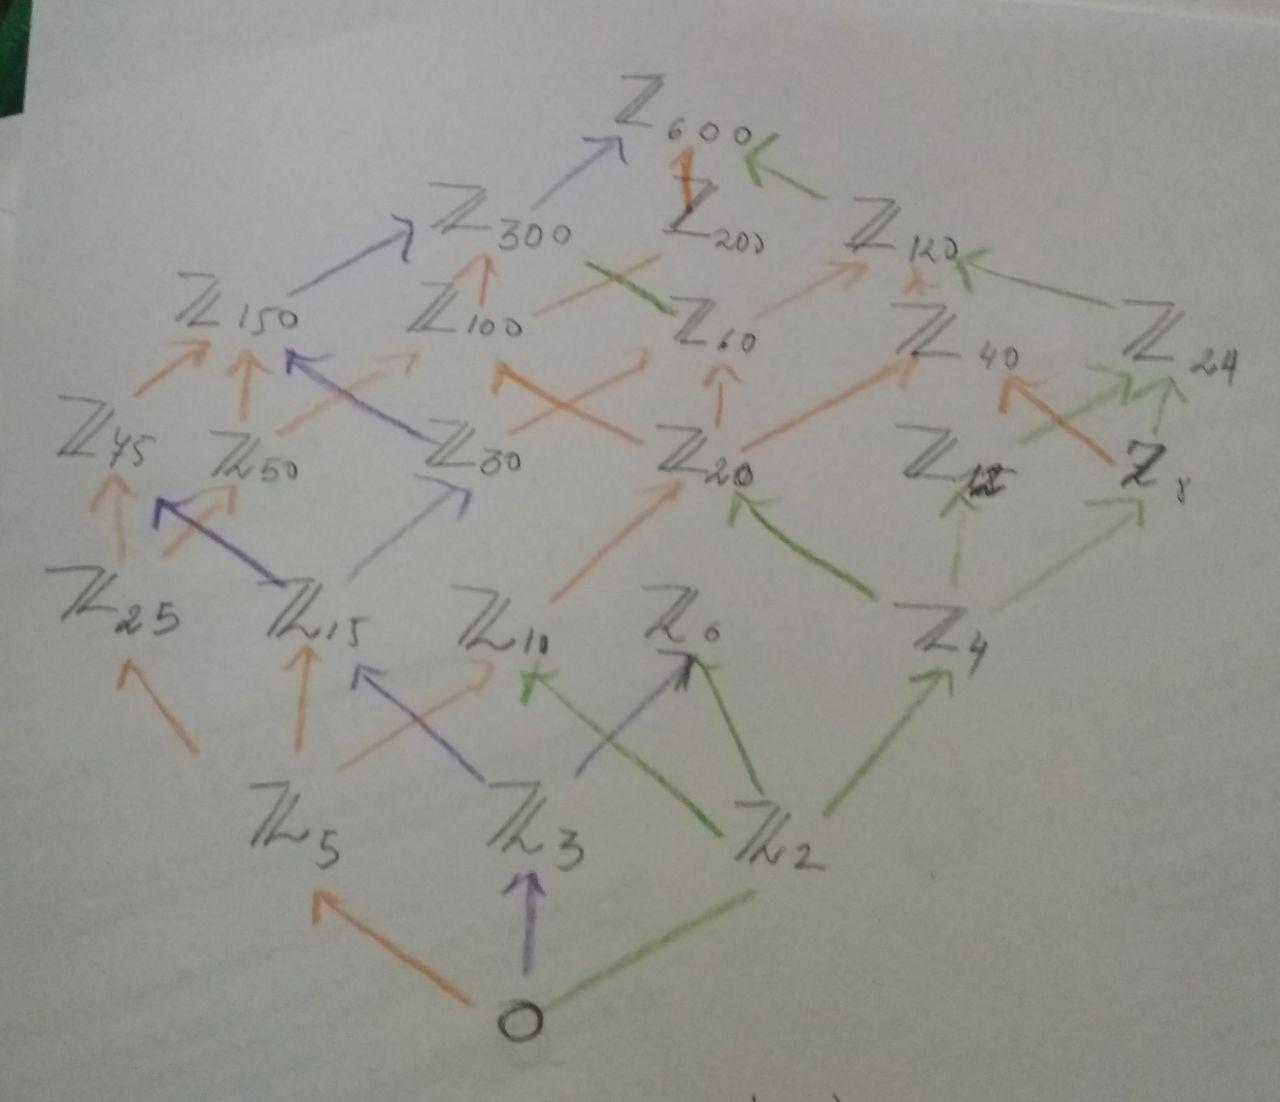
\includegraphics[width=\textwidth]{Z600}

\subsection{Tercer apartado}

\begin{micaja}
    Consideramos las permutaciones de $S_9,$
    $\sigma = (2 6)(132859)(263)$ y $\tau = (6734)(46)(37).$
    Demostrad que el subgrupo generado por ellas $<\sigma, \tau>,$ es cíclico. 
    Determine su orden y uno de sus generadores. 
\end{micaja}

Lo primero que vamos a hacer es espresar $\sigma$ y $\tau$ como ciclos disjuntos: 
\begin{itemize}
    \item $\sigma = (13859),$ que es un ciclo de longitud (y por tanto orden) 5.
    \item $\tau = (4 7),$ que es un ciclo de longitud (y por tanto orden) 2.
\end{itemize}

Observar los órdenes de un permutación es muy interesante porque si $\beta$ es una permutación
de longitud $n$ entonces $\beta^n = 1.$

Además, supongamos ahora  $\alpha$  es una permutación o composición de
permutacionens que se puede descomponer como $alpha = a_0 a_1 ..a_r$ con $a_i$ ciclos 
disjuntos de longitud $l_i$, entonces se tiene que el $mcm(l_1,l_2..l_r)$ será el orden de la permutación,
ya que si $m = mcm(l_0, l_1,..,l_3)$  y además por ser $a_0, a_1,..,a_r$ disjuntos serán conmutativos
  se tendrá que 
$$\alpha ^m = (a_0 a_1 ..a_r)^m = a_0^m a_1^m..a_r^m = 1$$

Ya que $m$ es múltiplo de todos las longitudes y además será el orden por ser el mínimo 
número en cumplir eso. 

Y si además $l_0,l_1,...l_r$ son primos relativos, se tiene la siguiente
igualdad: 

$m_0 = mcm(l_1,..,l_r)$ (nótese que hemos quitado el primero, ni que tampoco hemos perdido
genarilidad, ya que son comnutativos podemos reordenar.)

Por tanto 
\begin{equation}
    \alpha^{m_0} = (a_0 a_1 ..a_r)^{m_0} = a_0^{m_0} a_1^{m_0}..a_r^{m_0} = a_0^{m_0}
\end{equation}



Puesto que $m_0$ será múltiplo de todos los $l_i$ salvo de $l_0.$ \paragraph{}


Y esto va a describir a las permutaciones que generen $<\alpha>$, 
ya que serán todas aquellas de la forma $s = a_0^{-L_0} a_1^{-L_1} a_r^{-L_r}$
con $L_i$ múltiplo de los $l_j$ salvo del i-ésimo y primo relativo con el resto de $L_j.$
Veamos que $<s> = <\alpha>.$

Si $\lambda = \prod_{i=0}^r Li$ se tentrá por (1) que para cualquier ciclo disjunto $a_i$

$$ a_i = s^{\frac{\lambda}{L_i}}$$
Con esto hemos probado que $<\alpha> \subseteq <s>.$ Para la otra inclusión, si 
$L_i= \prod_{i=0}^{i-1} l_i \prod_{i+1}^r l_i$ (que recordamos que eran primos relativos)
entonces el 
$$ord(<s>)= mcm(L_0,..., L_r) = L_i*l_i = mcm(l_0, l_1,..., l_r) = ord(<\alpha>)$$
para cualquier $i$ subíndice de los coeficientes. 

Por lo que concluimos que $$<\alpha> = <s>$$ y es un grupo cíclico. 

\subsubsection*{Nuestro caso particular}
Vamos a elegir los $L_i$ más simples, para $\sigma$ la longitud de $\tau$ y para 
$\tau$ la de $\sigma.$ 
Por tanto 
 $$\gamma = \sigma ^{-2} \tau ^{-5} = \sigma^{5-2}\tau  = (1 5 3 9 8)(4 7)$$ 
 Se tendrá que 
 $$<\gamma> = < \sigma, \tau>$$ Por tanto $< \sigma, \tau>$ \textbf{ será un grupo cíclico 
 y uno de sus generadores será} $\gamma.$
 
 Su \textbf{orden} será el mínimo común múltiplo de las longitudes de $\sigma$ y $tau$: 

 $$ord(< \sigma, \tau>) = mcm(ord(\sigma), ord(\tau)) = mcm (5,2) = 10.$$

\subsection{Cuarto apartado}

\begin{micaja}
    Sea $n \geq 2$ y $p \leq n$ un número primo. Demostrad que en $S_n$ los únicos elementos
    de orden $p$ son los productos de ciclos disjuntos de longitud $p.$ ¿Cuántos elementos de orden
    2 tiene $S_5$?
\end{micaja}


\textbf{Condición suficiente.}\paragraph{}
 Sea $s \in S_n$  una permutación de orden $p$, si $s$ es un ciclo entonces es eviendente. 
 Si no admitirá ser expresado como la composición de ciclos disjuntos $s = a_0..a_r$ que 
 tendrá respectivamente $l_0, ..., l_r$ órdenes, y por tanto $ord(a) = mcm(l_0,...,l_r)$
 pero claro el $ord(a) = p$ que es primo, entonces necesariamente $p = l_0 = ... = l_r.$ 


\textbf{Condición suficiente.}\paragraph{}
Por las consiceraciones sobre orden del apartado anterior, sabemos que para $s \in S_n$, 
descomponible en ciclos disjuntos de longitud $p;$ entonces su orden 
va a ser el mínimo común múltiplo del orden de sus ciclos disjuntos, pero como este es
siempre $p$ entonces el orden de $s$ es $p.$

\subsubsection*{Elementos de orden 2 en $S_5$}

En $S_5$ existe $\frac{5!}{3!} = 5\times 4 = 20$  ciclos de orden 2 diferentes. 

Y por el apartado anterior todos los elementos de orden 2 que existe serán producto de estos ciclo disjuntos, 
(sin que importe el orden a la hora de componer): 

De lo que deducimos que habrá elementos de orden dos: $2^{20} -1$

\newpage

\section{Ejercio 3}
\subsection{Apartadoo primero}

\begin{micaja}
    Sean las matrices de Heisenberg. 

    Demostar que $G$ es un grupo (con producto de matrices). ¿Es abeliano? ¿Es cíclico?
    ¿Es $H$ un subgrupo de $G$? En caso afirmativo, ¿Es normal en $G$?

    Probar que $f: \leftarrow \mathbb R$ defini como $f(A)=a+c$ es un homomorfismo de grupos 
\end{micaja}

\subsubsection*{G es un grupo.}

Por la caracterización de grupo debe cumplir: 

\begin{enumerate}
    \item \textbf{Existencia de un elemento neutro}, la matriz identidad pertenece a $G$ 
    (que por tanto es no vacío) y a demás es el elemento neutro. 
    \item \textbf{Propiedad asociativa.} El producto de matrices es asociativo, así que aquí 
    también lo será. 
    \item \textbf{Existencia de un elemento inverso} en $G$ para todo elemento de $G$. 
    Esto se ve fácilmente de la siquiente manera: 

    \begin{equation*}
        Sea A \in G \text{ y por tanto es de la forma } A = 
        \left(
        \begin{matrix}
            1 & a & b \\
            0 & 1 & c \\
            0 & 0 & 1
        \end{matrix}
        \right)
    \end{equation*}
    Con $a,b,c\in \mathbb{R}$

    Y queremos encontrar una matriz de la forma 
    \begin{equation*}
        B= \left(
        \begin{matrix}
            1 & x & y \\
            0 & 1 & z \\
            0 & 0 & 1
        \end{matrix}
        \right)
    \end{equation*}

    Con $x,y,z \in \mathbb{R}$ (incógnitas) que cumplan que $AB = 1$

    Por tanto lo único que nos faltaría ver es que el sistem que forman $x,y,z$ tiene solución, 
    
    las ecuaciona a las que da lugar son 

  \begin{equation*}
    \left\{
      \begin{array}{l}
         x + a = 0 \\
         y + az + b = 0 \\
         z +c = 0
      \end{array}
      \right.
  \end{equation*}


Que tienen como sulución $x = -a, z = -c, y = ac-b$
que cumplen $x,y,z \in \mathbb{R}$ y como queriamos demostrar, 
para toda matriz de $G$ existe su inversa en $G.$

\end{enumerate}

\subsubsection*{Es abeliano}

El producto de matrices no es conmutativo en general, sin embargo para cualesquiera $A,B \in G$ 
se cumple que 

\begin{equation*}
    A B = 
    \begin{pmatrix}
        1 & a & b \\
        0 & 1 & c \\
        0 & 0 & 1
    \end{pmatrix}
    \times
    \begin{pmatrix}
        1 & x & y \\
        0 & 1 & z \\
        0 & 0 & 1
    \end{pmatrix}
    = 
    \begin{pmatrix}
    1 & x+a & y + az + b\\
    0 & 1 & z + c\\
    0 & 0 & 1
    \end{pmatrix}
\end{equation*}
\begin{equation*}
    = 
    \begin{pmatrix}
        1 & a+x & b+ za + y\\
        0 & 1 & c + z \\
        0 & 0 & 1
    \end{pmatrix}
 = \begin{pmatrix}
    1 & x & y \\
    0 & 1 & z \\
    0 & 0 & 1
\end{pmatrix}
\times  
 \begin{pmatrix}
    1 & a & b \\
    0 & 1 & c \\
    0 & 0 & 1
\end{pmatrix}
= B A
\end{equation*}

\subsubsection*{No es cíclico}


También podriamos haberlo visto por la numerabilidad de $\mathbb R$
(sí, confieso que he matado moscas a cañonazos).
Que fuera cíclico supondría que $\mathbb R$ es numerable, 
ya que si existera una matriz $E \in G$, 
de tal forma que $<E>=G$, necesariamente $E$ distinta de la identidad
entonces alguna de sus entradas correspondientes a $a,b,c$ serán no nulas 
, llamemos a la posición en la matriz de esta entrada $e$.
Pues bien si ahora, considera cualquier $r \in \mathbb R$, cogemos una matriz $R$
igual a la identidad salvo en $e$ que en vez de $0$, tiene en esa casilla $r.$

Sabemos que por ser un ciclo existiría un $n$ natural tal que $E^n = R$
y por tanto habriamos encontado una inyección de los reales en los naturales, lo cual
es un contradición. 

\subsubsection*{H es un subgrupo de G}
Esto será si para todo $X,Y \in H$ se cumple que $X Y^{-1} \in H$
Por el primer apartado hemos visto que si 

\begin{equation*}
    X = 
    \begin{pmatrix}
        1 & 0 & x \\
        0 & 1 & 0 \\
        0 & 0 & 1
    \end{pmatrix}
    Y = 
    \begin{pmatrix}
        1 & 0 & y \\
        0 & 1 & 0 \\
        0 & 0 & 1
    \end{pmatrix}
\end{equation*}
entonces la inversa $Y$ será de la forma: 

\begin{equation*}
    Y = 
    \begin{pmatrix}
        1 & 0 & -y \\
        0 & 1 & 0 \\
        0 & 0 & 1
    \end{pmatrix}
\end{equation*}

y finalente

\begin{equation*}
    XY^{-1} = 
    \begin{pmatrix}
        1 & 0 & x-y \\
        0 & 1 & 0 \\
        0 & 0 & 1
    \end{pmatrix}
\end{equation*}
Que es de las formas de las matrices de $H$, por lo que es un subgrupo.

\subsubsection*{Normalidad de H en G}

Es normal porque $G$ es conmutativo y por tanto 
para todo $a \in G$ se tendrá que $aH = Ha$

\subsubsection*{f es un homomorfismo de grupos}

Para que sea homomorfismo debe cumplir 
\begin{enumerate}
    \item \textbf{ La aplicación f lleva elementos neutros en elementos neutros}.
    El elemento neutro de $G$ es la matriz identidad la cual todas sus entradas
    menos la diagonal son ceros. 

    El elemento neutro de $(R,+)$ es el $0.$

    Y por último tenemos que $f(Id) = 0+0 = 0.$

    \item Por último habría que ver que $f(AB) = f(A)f(B)$ 
    para cualesquiera matrices $A,B \in G.$

    \begin{equation*}
        f(A)+ f(B)= 
        f 
    %    \left\( 
        \begin{pmatrix}
            1 & a &  b\\
            0 & 1 & c\\
            0 & 0 & 1
            \end{pmatrix}
           % \right\) 
           +
            f %\left\( 
        \begin{pmatrix}
            1 & x & y \\
            0 & 1 & z \\
            0 & 0 & 1
            \end{pmatrix}
            %\right\)
            = (a+c)+(x + z) 
    \end{equation*}
    y por otro lado
    \begin{equation*}
        f(AB)= 
        f %\left\( 
        \begin{pmatrix}
            1 & x+a & y + az + b\\
            0 & 1 & z + c\\
            0 & 0 & 1
            \end{pmatrix}
            %\right\) 
            = (x+a)+(z+c) 
    \end{equation*}
    
    Ambas expresiones son iguales por tanto es un homomorfismo. 
\end{enumerate}

\subsubsection*{Núcleo de f}

Se define el $ker(f)$  como   $ker(f) = \left\{ e \in G | f(e) = 0\right\}$
luego 
\begin{equation*}
    ker(f) = \left\{ \begin{pmatrix}
        1 & a & b \\
        0 & 1 & -a \\
        0 & 0 & 1
        \end{pmatrix} \text{ con  } a,b \in \mathbb R\right\}
\end{equation*}

\subsubsection*{Imagen de f}
REDACTAR MEJOR
Es todo $R$, bastará con ver que cierto conjunto de $G$
su imagen ya es $R.$

Dada una matriz de $G$ fijamos $a$ arbitrariamente
y por cómo está definida $c$ podrá ser cualquier real  por tanto 


\subsubsection*{No es monormorfismo}
Ya que su núcleo no es la identidad.

\subsubsection*{Es epimorfismo}
Ya que $Img(f) = \mathbb R$

\newpage
\subsection{Segundo apartado}

\begin{micaja}
    Sea $f:S_4 \rightarrow S_6$ la aplicación dada por
    $f(\sigma) = \bar \sigma$, donde $\bar \sigma$
    es el elemento de $S_6$ que actúa igual que $\sigma$
    sobre los elementos $\{1,2,3,4\}$ y sobre los elementos
    $\{5,6\}$ los fija se $\sigma$ es par, o los intercambia
    si $\sigma$ es impar.

    Demostad que $f$ es un homomorfismos 
    inyectivo de grupos y que su imagen está contenida en $A_6.$
\end{micaja}

\end{document}